\documentclass[aspectratio=169]{beamer}
%\documentclass{beamer}
\usetheme{LU-spfaff}
\usepackage[spanish]{babel}
\usepackage[utf8]{inputenc}
\usepackage[T1]{fontenc}

\setbeamercovered{invisible} % Velos
\usepackage{color}
\usepackage[spanish]{babel}
\usefonttheme{serif}

%%% Rellenos texto pruebas
\usepackage{lipsum}

%%% Figuras en formato .png, .ps, pdf, gif, jpg o eps
\usepackage{graphicx}
\usepackage{subfigure}
\DeclareGraphicsExtensions{.png,.eps,.ps,.pdf,.gif,.jpg}

%%% Soporte graficos svg
\usepackage{svg}


%%% COMANDOS  %%%
%%% COMANDOS  %%%

%%% A cursiva  %%%
\newcommand{\cursiva}[1]{\em{#1}}


%%% Fuzzing en bonito  %%%
\newcommand{\fz}{\em fuzzing}

%%% Atajos estilo  %%%

\newcommand{\CLASSINPUTinnersidemargin}{18mm}
\newcommand{\CLASSINPUToutersidemargin}{12mm}
\newcommand{\CLASSINPUTtoptextmargin}{20mm}
\newcommand{\CLASSINPUTbottomtextmargin}{25mm}

\newcommand{\new}[1]{\textcolor{olive}{{#1}}}
%\newcommand{\old}[1]{\textcolor{purple}{{\sout{#1}}}}
\newcommand{\wip}[1]{\textcolor{blue}{{#1}}}
%\newcommand{\checkthis}[1]{\textcolor{orange}{{#1}}}
\newcommand{\diego}[1]{\textcolor{magenta}{{#1}}}
\newcommand{\vmodixit}[1]{\textcolor{teal}{{#1}}}

\newcommand{\old}[1]{\textcolor{purple}{{\sout{#1}}}}
\newcommand{\camino}[1]{\textcolor{olive}{{#1}}}
\newcommand{\fjrodl}[1]{\textcolor{blue}{{#1}}}
\newcommand{\checkthis}[1]{\textcolor{orange}{{#1}}}

%%% Entornos  %%%
\newcounter{definicion}
\newenvironment{definicion}[1]{%
    \refstepcounter{definicion}\par\medskip%
    \noindent \textbf{Definición~\thedefinicion. #1}.\ %
}{\medskip}

%%%% Soporte para el logo de ORCID
%\newcommand{\orcid}[1]{\href{https://orcid.org/#1}{\textcolor[HTML]{A6CE39}{\aiOrcid}}}



%%% Paquete para usar símbolos y scripts de dibujado
\usepackage{tikz}
\def\checkmark{\tikz\fill[scale=0.4](0,.35) -- (.25,0) -- (1,.7) -- (.25,.15) -- cycle;} 
\usetikzlibrary{shapes,arrows}

% Define Block styles
\tikzstyle{decisionBL} = [diamond, draw, fill=blue!20,text width=10em, text badly centered, node distance=3cm, inner sep=0pt]
\tikzstyle{blockBL} = [rectangle, draw, fill=blue!20,text width=9em, text centered, rounded corners, minimum height=4em]
\tikzstyle{blockYL} = [rectangle, draw, fill=yellow!20, text width=9em, text centered, rounded corners, minimum height=4em]
\tikzstyle{blockGR} = [rectangle, draw, fill=green!20, text width=9em, text centered, rounded corners, minimum height=4em]
\tikzstyle{blockRD} = [rectangle, draw, fill=red!20, text width=9em, text centered, rounded corners, minimum height=4em]
\tikzstyle{blockWH} = [rectangle, draw, fill=white!20, text width=9em, text centered, rounded corners, minimum height=4em]
\tikzstyle{line} = [draw, -latex']
\tikzstyle{cloud} = [draw, ellipse,fill=red!20, node distance=4.5cm,minimum height=4em]

%%% Para usar ficheros tex de infografias Inkscape
\usepackage{pstricks}


%%% CAJAS  %%%
\usepackage{tcolorbox} 
\tcbuselibrary{skins,theorems}
\tcbset{
cajaRG/.style={
  beamer,
  colback=white,
  colbacktitle=white,
  coltitle=red!70!black,
  colframe=white,
  boxrule=1pt,
  titlerule=0pt,
  arc=15pt,
  middle=0pt,
  boxsep=0pt,
  borderline={0.5pt}{0.2pt}{red},
  theorem name,
  description delimiters=(),
  title={\strut#1}
  }
}
\newtcbtheorem{CJdef}{Definición}{cajaRG}{thm}
\newtcbtheorem{CJxxx}{}{cajaRG}{thm}



% % % % % % % % % % % % % % % % % % % % % % % % % % % % % % % % % % % % % % % % % % %

%\title[HOUSE: fuzzing en HPC]{%
\title[HOUSE]{%
% ** (TÍTULO LARGO) **
HOUSE: Marco de trabajo modular de arquitectura\\%
escalable y desacoplada para el uso de técnicas de\\%
{\fz} en HPC\\%
% ** (AUTORES) **
\small{\underline{Francisco Borja Garnelo Del Río}, Francisco J. Rodríguez Lera,}\\
\small{Gonzalo Esteban Costales, Camino Fernández Llamas,}\\
\small{Vicente Matellán Olivera}\\
% ** (AFILIACIÓN) **
\small{\textit{Universidad de León}}
}

\titlecolor{LUWhite} % Choose between LUPink, LULBlue, LUIvory, LUGreen
\titleimage{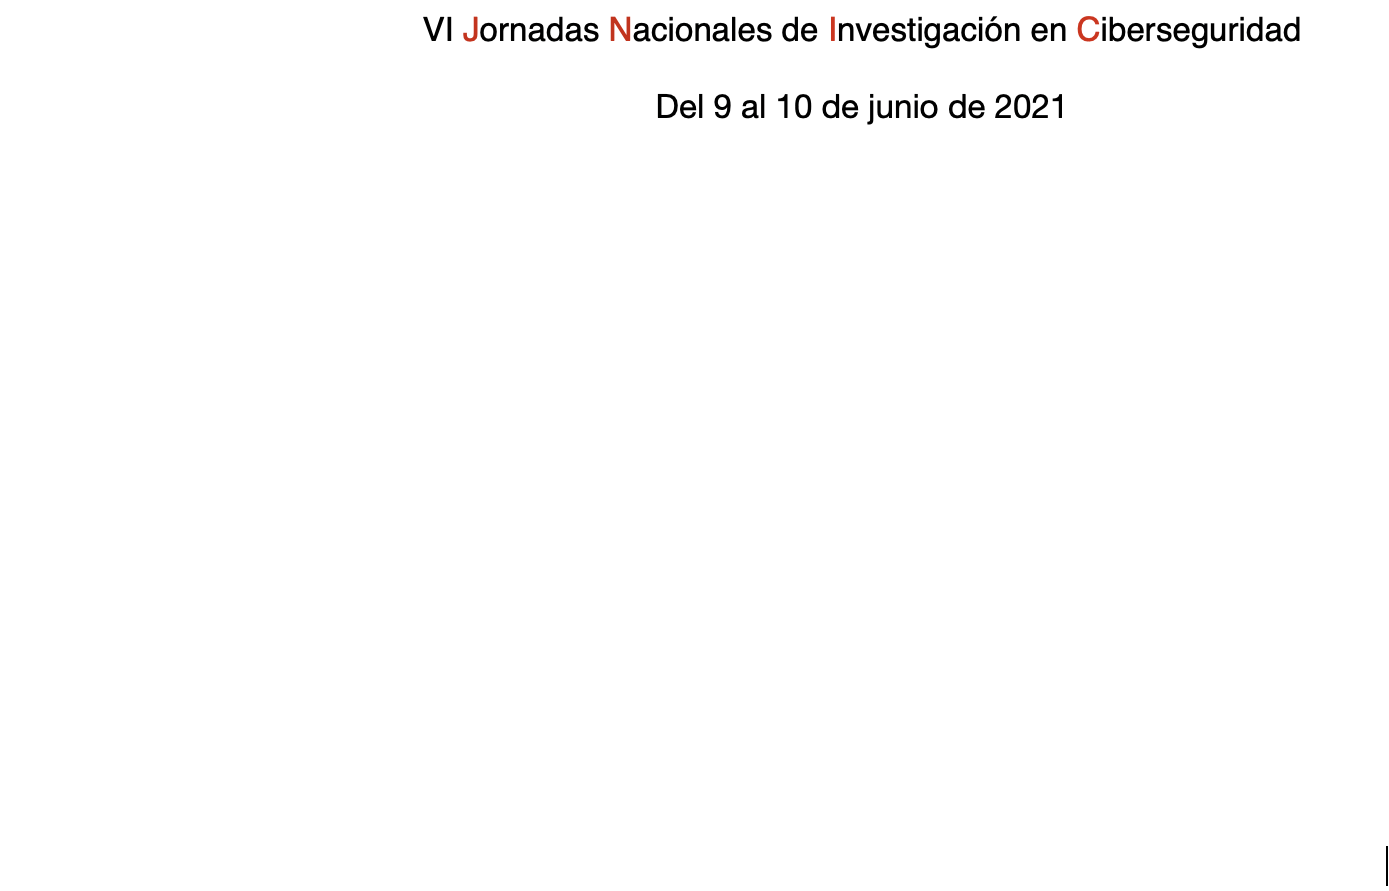
\includegraphics[scale=0.55]{./img/jornadas.png}}

% ** (CORRESPONDING AUTHOR) **
% Otra opción para que no te coma tanto espacio en la parte de abajo de las
% diapositivas puede ser poner: \author{F.B. Garnelo del Río (infbgd01@estudiantes.unileon.es)}
% Así podrías poner el título "corto" de la presentación algo más largo (te lo he dejado comentado)
%\author{Francisco Borja Garnelo Del Río (infbgd01@estudiantes.unileon.es)}
\author{Francisco B. Garnelo del Río (infbgd01@estudiantes.unileon.es)}

\date{JNIC LIVE 2021}

\begin{document}
\renewcommand{\contentsname}{Contenidos}
\renewcommand{\figurename}{Figura}
\renewcommand{\tablename}{Tabla}
\renewcommand{\sectionname}{Sección}
\renewcommand{\subsectionname}{Subsección}
\renewcommand{\partname}{Parte}

% *** TÍTULO ***
\titleframe

% *** ÍNDICE ***
\begin{frame}[noframenumbering]{Índice de contenidos}
    \tableofcontents
\end{frame}
 
% ***************************************************************************
%%% PRUEBAS ESTILOS Y FORMAS
\iffalse % DESHABILITA LAS PRUEBAS
%\iftrue % HABILITA LAS PRUEBAS
\section{PRUEBAS}
\frame{\sectionpage}

\begin{frame}{Motivación}


    \only<1>{

        \begin{columns}

            \begin{column}{0.45\textwidth}
                El {\fz}~\cite{contexto_fuzzing} es la automatización de generación y prueba de entradas malformadas en el software con el fin de encontrar comportamientos no esperados en el mismo, habitualmente \textit{crashes}%
                \footnote{\textbf{\textit{crash}}~\cite{IEEE_SW_standar}
                Fallo repentino y completo de un sistema o componente informático.
                }. %
            \end{column}

            \begin{column}{0.45\textwidth}
        \includesvg{./img/Infografia_CASA_paper.svg}
     
            \end{column}
        \end{columns}
        

    }


    \only<2>{
    
    %%%% Ejemplo cajas

\begin{CJdef}{}{test1}
test1
\end{CJdef}
\begin{CJdef}{lolo}{test2}
test2
\end{CJdef}

\newtcbtheorem{CJprueba}{Prueba}{cajaRG}{test3}
\begin{CJprueba}{}{testc}
test
\end{CJprueba}
\begin{CJxxx}{lala}{test4}
test
\end{CJxxx}

    }


    \only<3>{
    %%%% Ejemplo items y numeración
        \begin{itemize}
            \item LOLLA
                ADASD
            \item LLULUUL:
                \begin{enumerate}
                    \item chumba
                    \item sdf234
                    \item 53gv
                \end{enumerate}
        \end{itemize}

    }

    \only<4>{

%%% BLOQUES %%
%%% https://texdoc.org/serve/tcolorbox.pdf/0

        \begin{columns}

            \begin{column}{0.60\textwidth}
%%%    %%% https://texdoc.org/serve/tcolorbox.pdf/0 (Pag 13)
\tcbset{colback=green!10!white}
\tcbsetforeverylayer{colframe=red!75!black}
\begin{tcolorbox}[title=All options for this box]
This is a tcolorbox.\par\medskip
\begin{tcolorbox}[title=Nested box]
Note that this nested box has a red frame but no green background.
\end{tcolorbox}
\end{tcolorbox}
\bigskip
\begin{tcolorbox}[reset]
Options given with |\tcbsetforeverylayer| survive a |reset|.
\end{tcolorbox}
        \end{column}
 \end{columns}
    }

    \only<5>{

%%% BLOQUES %%
%%% https://texdoc.org/serve/tcolorbox.pdf/0

        \begin{columns}

            \begin{column}{0.45\textwidth}
%%%    %%% https://texdoc.org/serve/tcolorbox.pdf/0 (Pag 15)
\newtcolorbox{mybox}{colback=red!5!white,
colframe=red!75!black}
\begin{mybox}
This is my own box.
\end{mybox}
        \end{column}
                    \begin{column}{0.45\textwidth}
%%%    %%% https://texdoc.org/serve/tcolorbox.pdf/0 (Pag 15)
\newtcolorbox{mybox}[1]{colback=red!5!white,
colframe=red!75!black,fonttitle=\bfseries,
title=#1}
\begin{mybox}{Hello there}
This is my own box with a mandatory title.
\end{mybox}

        \end{column}
        
 \end{columns}
    }

    \only<6>{

%%% BLOQUES %%
%%% https://texdoc.org/serve/tcolorbox.pdf/0

        \begin{columns}

            \begin{column}{0.45\textwidth}
%%%    %%% https://texdoc.org/serve/tcolorbox.pdf/0 (Pag 435)
\tcbset{colback=red!5!white,
colframe=red!75!black,left=1mm,
right=1mm,boxsep=0mm}
\begin{tcolorbox}[fit to height=4cm]
{\Large\bfseries This text is
not adapted:\par}
Hola ke ases Hola ke ases Hola ke ases Hola ke ases Hola ke ases Hola ke ases

\end{tcolorbox}
\begin{tcolorbox}[fit to height=4cm,
fit fontsize macros ]
{\Large\bfseries This text is adapted:\par}
Hola ke ases Hola ke ases Hola ke ases Hola ke ases Hola ke ases Hola ke ases
Hola ke ases Hola ke ases Hola ke ases Hola ke ases Hola ke ases Hola ke ases
\end{tcolorbox}

        \end{column}
                    \begin{column}{0.45\textwidth}
%%%    %%% https://texdoc.org/serve/tcolorbox.pdf/0 (Pag 435)
\tcbset{colback=red!5!white,
colframe=red!75!black,left=1mm,
right=1mm,boxsep=0mm}
\let\realHuge=\Huge
\begin{tcolorbox}[fit basedim=7pt,
fontupper=\normalsize,
fit fontsize macros]
The relative font size macros
are also usable without the
\textit{fit} algorithm.\par
{\Huge Adapted Huge} ---
{\realHuge Original Huge}
\end{tcolorbox}
        \end{column}
        
 \end{columns}
    }

  \only<7>{

%%% BLOQUES %%
%%% https://texdoc.org/serve/tcolorbox.pdf/0

        \begin{columns}

            \begin{column}{0.45\textwidth}
%%%    %%% https://texdoc.org/serve/tcolorbox.pdf/0 (Pag 444)
\tcbset{colback=red!5!white,colframe=red!75!black,fonttitle=\bfseries}
\begin{tcolorbox}[title=My title,before app={The box follows:\\[4pt]},
after app={This is the end.}]
This is a \textbf{tcolorbox}.
\end{tcolorbox}


        \end{column}
                    \begin{column}{0.45\textwidth}
%%%    %%% https://texdoc.org/serve/tcolorbox.pdf/0 (Pag 470)


        \end{column}
        
 \end{columns}
    }

\only<8>{

\begin{block}{Título}
Test 1
\end{block}

\begin{alertblock}{Título}
Test 1
\end{alertblock}

\begin{exampleblock}{Título}
Test 1
\end{exampleblock}

}
\end{frame}
\fi

\section{Introducción}
\frame{\sectionpage}

\begin{frame}{Motivación}

% ---- DIAPOSITIVA ----
% * Describir qué es fuzzing
% * Enumerar los problemas actuales relativos a usar fuzzing
% ---------------------
        \only<1>{

        \begin{CJdef}{{\fz}~\cite{contexto_fuzzing}}
.La automatización de generación y prueba de entradas malformadas en el software con el fin de encontrar comportamientos no esperados en el mismo. 
\end{CJdef}
        
        \begin{itemize}
 % \item El {\fz} es la automatización de generación y prueba de entradas malformadas en el software con el fin de encontrar comportamientos no esperados en el mismo~\cite{contexto_fuzzing}, habitualmente fallos repentinos y completos de un sistema o componente informático como crashes~\cite{IEEE_SW_standar}.\\
\item Habitualmente fallos repentinos y completos de un sistema o componente informático conocidos como crashes~\cite{IEEE_SW_standar}.
%\item  Este término se usó por primera vez en un estudio de la seguridad de UNIX en la década de 1990~\cite{inicio_fuzzing,continuacion_fuzzing}.
        \end{itemize}
        \begin{CJdef}{HPC, high-performance computing}
.Computación de alto rendimiento o supercomputación.
\end{CJdef}
}

  \only<2>{
  \begin{itemize}
    \item Los problemas identificados en la literatura:
     \begin{enumerate}
  \item Complejidad de modificar una parte sin tener que montar algo complejo para ello (técnicas y herramientas).
  \item Monopolio de las herramientas y confidencialidad de los datos.
  \item Dificultad, especialización y puesta en marcha (aplicación práctica).
  \end{enumerate}
  \end{itemize}      
  }


\end{frame}
\begin{frame}{Objetivos}
%\begin{itemize}
%    \item Los principales objetivos de esta investigación son:
\begin{enumerate}
    \item Conocer el estado actual del {\fz} enfocándolo a su uso en entornos HPC.
    \item Dar una visión global de las actividades previas, los procesos y componentes del {\fz} respecto a las últimas mejoras y las adaptaciones a entornos de computación escalable.
\end{enumerate}            
%\end{itemize}      


% ---- DIAPOSITIVA ----
% * Presentar los 2 objetivos del artículo
% ---------------------

\end{frame}

% ***************************************************************************
\section{Trabajo relacionado}
\frame{\sectionpage}

\begin{frame}{Tipos de pruebas de seguridad en el software~\cite{fuzz_ref_sec-qa_sw}}

% ---- DIAPOSITIVA ----
% * Mencionar los que comentas en el paper: activas/dinámicas y pasivas/estáticas
% * Dar definiciones y algún ejemplo (pero muy poca cosa)
% ---------------------
%En base a su naturaleza y enfoque las para identificar comportamientos no esperados pueden ser:
 \begin{itemize}
  \item \textbf{Activas o dinámicas}, implican la ejecución total o parcial del software.
   \begin{itemize}
    \item \textbf{Proactivas}, automatizan la ejecución de forma instrumentada con herramientas de {\fz} (BFF, radamsa o AFL).
    \item \textbf{Reactivas}, observan el comportamiento del software en un entorno de producción (SELinux o EPDR).
   \end{itemize} 
  \item  \textbf{Pasivas o estáticas}, no implican la ejecución del software, habitualmente emplean el código fuente (CodeQL, Sonarqube, Yasca o Flawfinder).
 \end{itemize}


\end{frame}

\begin{frame}{Tipos de fuzzing~\cite{fuzz_ref_sec-qa_sw}}

% ---- DIAPOSITIVA ----
% * Mencionar los que comentas en el paper: white-box, black-box y grey-box
% * Igual que antes, dar definiciones y algún ejemplo (pero muy poca cosa)
% ---------------------
 \begin{itemize}
 \item Se clasifican en función de los detalles de la implementación disponible.

 \begin{itemize}
 \item \textit{\textbf{white-box} {\fz}}, parte del código fuente.
 \item \textit{\textbf{black-box} {\fz}}, utiliza el software ya compilado en formato binario.
 \end{itemize}

 \item Entre estos dos tipos se situaría un tercero:
 \begin{itemize}
  \item \textit{\textbf{grey-box} {\fz}}, combina características de ambos, como es el caso de las pruebas donde se utiliza instrumentación en el código fuente y el análisis BVA.
 \end{itemize}
 \end{itemize}

\end{frame}

% ***************************************************************************
\section{Marco de trabajo HOUSE}
%%% Hacer hincapié aquí.

\frame{\sectionpage}

\begin{frame}{HOUSE}

\only<1>{
% ---- DIAPOSITIVA ----
% * Definición ¿Que es HOUSE? y características.
% * Diagrama de flujo (4 fases del fuzzing) el del paper y su descripción.
% ---------------------
\newtcolorbox{mybox}{colback=red!5!white,
colframe=red!75!black}
\begin{mybox}
Marco de trabajo con un enfoque funcional que facilita la coherencia y continuidad de forma global abordando el {\fz} como un flujo con distintas \textbf{fases}, organizando todos los procesos implicados, incluyendo también aquellos con relación directa.
\newline
 \begin{itemize}
  \item Modular.
  \item Abierto.
  \item Agnóstico a las herramientas y técnicas.
 \end{itemize}
\end{mybox}
}
\end{frame}

\begin{frame}{Fases del {\fz}}

\only<1>{
        \begin{columns}
            \begin{column}{0.40\textwidth}
\begin{enumerate}
    \item \textbf{Común} \textit{o de preparación del entorno de trabajo}.
    \item \textbf{\textit{Prefuzzing}} \textit{o de preparación de las pruebas software.}
    \item \textbf{\textit{Fuzzing}}\textit{ o de ejecución de las propias pruebas.}
    \item \textbf{\textit{Postfuzzing}}\textit{ o de análisis de resultados y tareas posteriores.}
\end{enumerate}
        \end{column}
                    \begin{column}{0.50\textwidth}

\begin{figure}[!ht]
  \centering
  % centering debería centrar adecuadamente la figura, así que, por norma general, no es necesario utilizar hspace
  %\hspace*{-135pt}
  \begin{tikzpicture}[node distance = 2cm, auto,
  % En un paper, las figuras suelen tener una fuente de tipo sin serifa (para
  % distinguirlas del texto). Además, todos elementos de texto deberían tener
  % el mismo tamaño de fuente)
  font=\large\sffamily,
  % Estas dos opciones de tikzpicture son para poder reescalar la imagen
  transform shape, scale=0.40
  ]
    % nodes
    \node [blockWH] (prep_env) {Preparar entorno de trabajo};
    \node [decisionBL, below of = prep_env, node distance = 3.5cm] (Hay_src) {¿Hay código fuente disponible?};
    \node [blockBL, right of = Hay_src, node distance = 5cm] (prep_src) {Preparar código fuente};
    \node [blockBL, below of = Hay_src, node distance = 3.5cm] (prep_bin) {Preparar binarios};
    \node [blockBL, below of = prep_bin, node distance = 2cm] (prep_in) {Preparar entradas};
    \node [blockGR, below of = prep_in, node distance = 2cm] (pruebas) {Paquete de trabajo de fuzzing};
    \node [blockYL, below of = pruebas, node distance = 2.3cm] (resultados) {Analizar resultados de los paquetes de trabajo};

    % edges
    \path [line] (prep_env) -- (Hay_src);
    \path [line] (Hay_src) -- node[midway,above] {Sí} (prep_src);
    \path [line] (Hay_src) -- node[midway,right] {No}(prep_bin);
    \path [line] (prep_bin) -- (prep_in);
    \path [line] (prep_src) |- (prep_bin);
    \path [line] (prep_in) -- (pruebas);
    \path [line] (pruebas) -- (resultados);

  % Leyenda cuqui
  \node [left of={prep_env},xshift=-2cm,blockWH,rotate=90,text width=2.2cm] (center:Common) {Común};
  \node [left of={prep_bin},xshift=-2cm,yshift=1.32cm,blockBL,rotate=90,text width=8.5cm] (center:Prefuzzing) {Prefuzzing};
  \node [left of={pruebas},xshift=-2cm,yshift=-0.11cm,blockGR,rotate=90,text width=1.8cm] (center:Fuzzing) {Fuzzing};
  \node [left of={resultados},xshift=-2cm,yshift=-0.1cm,blockYL,rotate=90,text width=2.2cm] (center:Postfuzzing) {Postfuzzing};

  %\node [above of={center:Common}] {Phases/Steps};

  \end{tikzpicture}
  %\caption{ Diagrama de flujo para describir el funcionamiento de HOUSE según las diferentes fases de fuzzing. }
  \label{fig:HOUSE_flow}
\end{figure}

        \end{column}
        
 \end{columns}
}

%%% Detalles fase recorte por tiempo.
\iffalse % DESHABILITA LOS DETALLES
%\iftrue % HABILITA LOS DETALLES

\only<2>{
        \begin{columns}
            \begin{column}{0.40\textwidth}
\begin{enumerate}\setcounter{enumi}{0}
    \item \textbf{Común o de preparación del entorno de trabajo}.
    Es la única fase transversal a todo el proceso ya que se suele realizar una única vez, bien en la puesta en marcha de las herramientas necesarias para el {\fz} o bien durante el despliegue inicial del marco de trabajo.
\end{enumerate}
        \end{column}
                    \begin{column}{0.50\textwidth}

\begin{figure}[!ht]
  \centering
  % centering debería centrar adecuadamente la figura, así que, por norma general, no es necesario utilizar hspace
  %\hspace*{-135pt}
  \begin{tikzpicture}[node distance = 2cm, auto,
  % En un paper, las figuras suelen tener una fuente de tipo sin serifa (para
  % distinguirlas del texto). Además, todos elementos de texto deberían tener
  % el mismo tamaño de fuente)
  font=\large\sffamily,
  % Estas dos opciones de tikzpicture son para poder reescalar la imagen
  transform shape, scale=0.45
  ]
    % nodes
    \node [blockWH] (prep_env) {Preparar entorno de trabajo};
    \node [decisionBL, below of = prep_env, node distance = 3.5cm] (Hay_src) {¿Hay código fuente disponible?};
  

    % edges
    \path [line] (prep_env) -- (Hay_src);

  % Leyenda cuqui
  \node [left of={prep_env},xshift=-2cm,blockWH,rotate=90,text width=2.2cm] (center:Common) {Común};


  %\node [above of={center:Common}] {Phases/Steps};

  \end{tikzpicture}
  %\caption{ Diagrama de flujo para describir el funcionamiento de HOUSE según las diferentes fases de fuzzing. }
  \label{fig:HOUSE_flow}
\end{figure}

        \end{column}
        
 \end{columns}
}

\only<3>{
        \begin{columns}

            \begin{column}{0.40\textwidth}
\begin{enumerate}\setcounter{enumi}{1}
    \item \textbf{\textit{Prefuzzing} o de preparación de las pruebas software}.
    En esta fase se elige el tipo de {\fz} a utilizar en función del grado de acceso y las necesidades de adaptación del código fuente.  En función del tipo elegido, se preparan los binarios correspondientes, también se confecciona o valida un conjunto de entradas para esa campaña de {\fz}~\cite{fuzzing_SOA}.
\end{enumerate}
        \end{column}
                    \begin{column}{0.50\textwidth}

\begin{figure}[!ht]
  \centering
  % centering debería centrar adecuadamente la figura, así que, por norma general, no es necesario utilizar hspace
  %\hspace*{-135pt}
  \begin{tikzpicture}[node distance = 2cm, auto,
  % En un paper, las figuras suelen tener una fuente de tipo sin serifa (para
  % distinguirlas del texto). Además, todos elementos de texto deberían tener
  % el mismo tamaño de fuente)
  font=\large\sffamily,
  % Estas dos opciones de tikzpicture son para poder reescalar la imagen
  transform shape, scale=0.45
  ]
    % nodes
    \node [decisionBL, below of = prep_env, node distance = 3.5cm] (Hay_src) {¿Hay código fuente disponible?};
    \node [blockBL, right of = Hay_src, node distance = 5cm] (prep_src) {Preparar código fuente};
    \node [blockBL, below of = Hay_src, node distance = 3.5cm] (prep_bin) {Preparar binarios};
    \node [blockBL, below of = prep_bin, node distance = 2cm] (prep_in) {Preparar entradas};
    \node [blockGR, below of = prep_in, node distance = 2cm] (pruebas) {Paquete de trabajo de fuzzing};


    % edges
     \path [line] (Hay_src) -- node[midway,above] {Sí} (prep_src);
    \path [line] (Hay_src) -- node[midway,right] {No}(prep_bin);
    \path [line] (prep_bin) -- (prep_in);
    \path [line] (prep_src) |- (prep_bin);
    \path [line] (prep_in) -- (pruebas);


  % Leyenda cuqui
  \node [left of={prep_bin},xshift=-2cm,yshift=1.32cm,blockBL,rotate=90,text width=8.5cm] (center:Prefuzzing) {Prefuzzing};


  %\node [above of={center:Common}] {Phases/Steps};

  \end{tikzpicture}
  %\caption{ Diagrama de flujo para describir el funcionamiento de HOUSE según las diferentes fases de fuzzing. }
  \label{fig:HOUSE_flow}
\end{figure}

        \end{column}
        
 \end{columns}
}

\only<4>{
        \begin{columns}

            \begin{column}{0.40\textwidth}
\begin{enumerate}\setcounter{enumi}{2}
    \item \textbf{\textit{Fuzzing} o de ejecución de las propias pruebas}.
    Fase en la que se somete el software bajo prueba (PUT - \textit{Program Under Test}) al {\fz} utilizando la configuración realizada previamente.
\end{enumerate}
        \end{column}
                    \begin{column}{0.50\textwidth}

\begin{figure}[!ht]
  \centering
  % centering debería centrar adecuadamente la figura, así que, por norma general, no es necesario utilizar hspace
  %\hspace*{-135pt}
  \begin{tikzpicture}[node distance = 2cm, auto,
  % En un paper, las figuras suelen tener una fuente de tipo sin serifa (para
  % distinguirlas del texto). Además, todos elementos de texto deberían tener
  % el mismo tamaño de fuente)
  font=\large\sffamily,
  % Estas dos opciones de tikzpicture son para poder reescalar la imagen
  transform shape, scale=0.45
  ]
    % nodes
    \node [blockGR, below of = prep_in, node distance = 2cm] (pruebas) {Paquete de trabajo de fuzzing};
    \node [blockYL, below of = pruebas, node distance = 2.3cm] (resultados) {Analizar resultados de los paquetes de trabajo};

    % edges
    \path [line] (pruebas) -- (resultados);

  % Leyenda cuqui
  \node [left of={pruebas},xshift=-2cm,yshift=-0.11cm,blockGR,rotate=90,text width=1.8cm] (center:Fuzzing) {Fuzzing};

  %\node [above of={center:Common}] {Phases/Steps};

  \end{tikzpicture}
  %\caption{ Diagrama de flujo para describir el funcionamiento de HOUSE según las diferentes fases de fuzzing. }
  \label{fig:HOUSE_flow}
\end{figure}

        \end{column}
        
 \end{columns}
}

\only<5>{
        \begin{columns}

            \begin{column}{0.40\textwidth}
\begin{enumerate}\setcounter{enumi}{3}
    \item \textbf{\textit{Postfuzzing} o de análisis de resultados y tareas posteriores}.
    En esta última fase, bien si se desea o bien si por volumen de trabajo es necesario automatizar la tarea de análisis de resultados, es posible ejecutar un paquete de trabajo creado expresamente para poner en valor los resultados del {\fz}.
\end{enumerate}
        \end{column}
                    \begin{column}{0.50\textwidth}

\begin{figure}[!ht]
  \centering
  % centering debería centrar adecuadamente la figura, así que, por norma general, no es necesario utilizar hspace
  %\hspace*{-135pt}
  \begin{tikzpicture}[node distance = 2cm, auto,
  % En un paper, las figuras suelen tener una fuente de tipo sin serifa (para
  % distinguirlas del texto). Además, todos elementos de texto deberían tener
  % el mismo tamaño de fuente)
  font=\large\sffamily,
  % Estas dos opciones de tikzpicture son para poder reescalar la imagen
  transform shape, scale=0.45
  ]
    % nodes

    \node [blockYL, below of = pruebas, node distance = 2.3cm] (resultados) {Analizar resultados de los paquetes de trabajo};

    % edges
    \path [line] (pruebas) -- (resultados);

  % Leyenda cuqui
  \node [left of={resultados},xshift=-2cm,yshift=-0.1cm,blockYL,rotate=90,text width=2.2cm] (center:Postfuzzing) {Postfuzzing};

  %\node [above of={center:Common}] {Phases/Steps};

  \end{tikzpicture}
  %\caption{ Diagrama de flujo para describir el funcionamiento de HOUSE según las diferentes fases de fuzzing. }
  \label{fig:HOUSE_flow}
\end{figure}

        \end{column}
        
 \end{columns}
}
\fi  %%% Detalle de fase, recortado por tiempo.
\end{frame}


\begin{frame}{Módulos de HOUSE}

% ---- DIAPOSITIVA ----
% * ¿Dibujo casa? (para explicar los paquetes/módulos), para comentar los módulos.
% ---------------------
%%% Estilo caja módulos
\newtcolorbox{CJmodulos}[1]{colback=red!5!white,colframe=red!75!black,fonttitle=\bfseries,title=#1}

\only<1>{

        \begin{columns}
\begin{column}{0.45\textwidth}
%\includesvg{./img/Infografia_CASA_paper.svg}

\begin{figure}[htbp]
   \centering
    \resizebox{1\textwidth}{!}{\includesvg{./figures/data/Infografia_CASA_paper.svg}} 
    %\caption{Infografía módulos marco de trabajo HOUSE.}
    \label{fig:infografia_modulos}
\end{figure}

   
        \end{column}
\begin{column}{0.45\textwidth}
El nombre de HOUSE hace referencia a la clásica metáfora~\cite{SW_ref_metafora} de describir un proceso como el diseño y construcción de una casa y, en este caso, describe el proceso de desarrollo seguro del software, pero desde el punto de vista del {\fz}.
    \end{column}
 \end{columns}
}

\only<2>{
\begin{CJmodulos}{\textit{Input Repository} (A.IR)}
Repositorio de entradas como semillas para generadores de entradas, diccionarios, archivos de muestra, etc.
\end{CJmodulos}

\begin{CJmodulos}{\textit{Output Repository} (B.OR)}
Repositorio de salidas con los contextos de ejecuciones de los \textit{fuzzers}, resultados, logs, etc.
\end{CJmodulos}

\begin{CJmodulos}{\textit{TooL Box} (0.TLB)}
 Colección de herramientas y utilidades auxiliares a cualquiera de las fases del {\fz}.
\end{CJmodulos}
}

\only<3>{
\begin{CJmodulos}{\textit{Source Code Integration} (1.SCI)}
Colección de códigos fuente, incluyendo parches, integraciones y optimizaciones previas al {\fz}.
\end{CJmodulos}

\begin{CJmodulos}{\textit{Binaries Ready to Fuzz} (2.BRF)}
Colección de binarios preparada para el {\fz}.
\end{CJmodulos}

\begin{CJmodulos}{\textit{WorkLoad Package} (3.WLP)}
Colección de paquetes con cargas de trabajo de cualquiera de las fases.
\end{CJmodulos}
}

%%% Cambio para más claridad
\iffalse % DESHABILITA MODULOS COMO LISTADO
%\iftrue % HABILITA MODULOS COMO LISTADO
\only<4>{
   \begin{itemize}
\item \textbf{\textit{TooL Box} (0.TLB)}.
    Colección de herramientas y utilidades auxiliares a cualquiera de las fases del {\fz}.

\item \textbf{\textit{Source Code Integration} (1.SCI)}.
    Colección de códigos fuente, incluyendo parches, integraciones y optimizaciones previas al {\fz}.
\item \textbf{\textit{Binaries Ready to Fuzz} (2.BRF)}.
    Colección de binarios preparada para el {\fz}.
\item \textbf{\textit{WorkLoad Package} (3.WLP)}.
    Colección de paquetes con cargas de trabajo de cualquiera de las fases.
\item \textbf{\textit{Input Repository}(A.IR)}.
    Repositorio de entradas como semillas para generadores de entradas, diccionarios, archivos de muestra, etc.
\item \textbf{\textit{Output Repository}(B.OR)}.
    Repositorio de salidas con los contextos de ejecuciones de los \textit{fuzzers}, resultados, logs, etc.
\end{itemize}          

}
\fi

\end{frame}

\begin{frame}{Flujo de trabajo: BPMN}

\only<1>{
\centering
% ---- DIAPOSITIVA ----
% * Diagrama BPMN global
% ---------------------
%\resizebox{1\textwidth}{!}{\includesvg{PresentacionJNIC/figures/data/Tabla_procesos_v5_ES.svg}}


%\resizebox{0.2\textwidth}{!}{\includesvg{./img/Tabla_procesos_v5_ES.svg}}
        \begin{columns}
\begin{column}{1\textwidth}
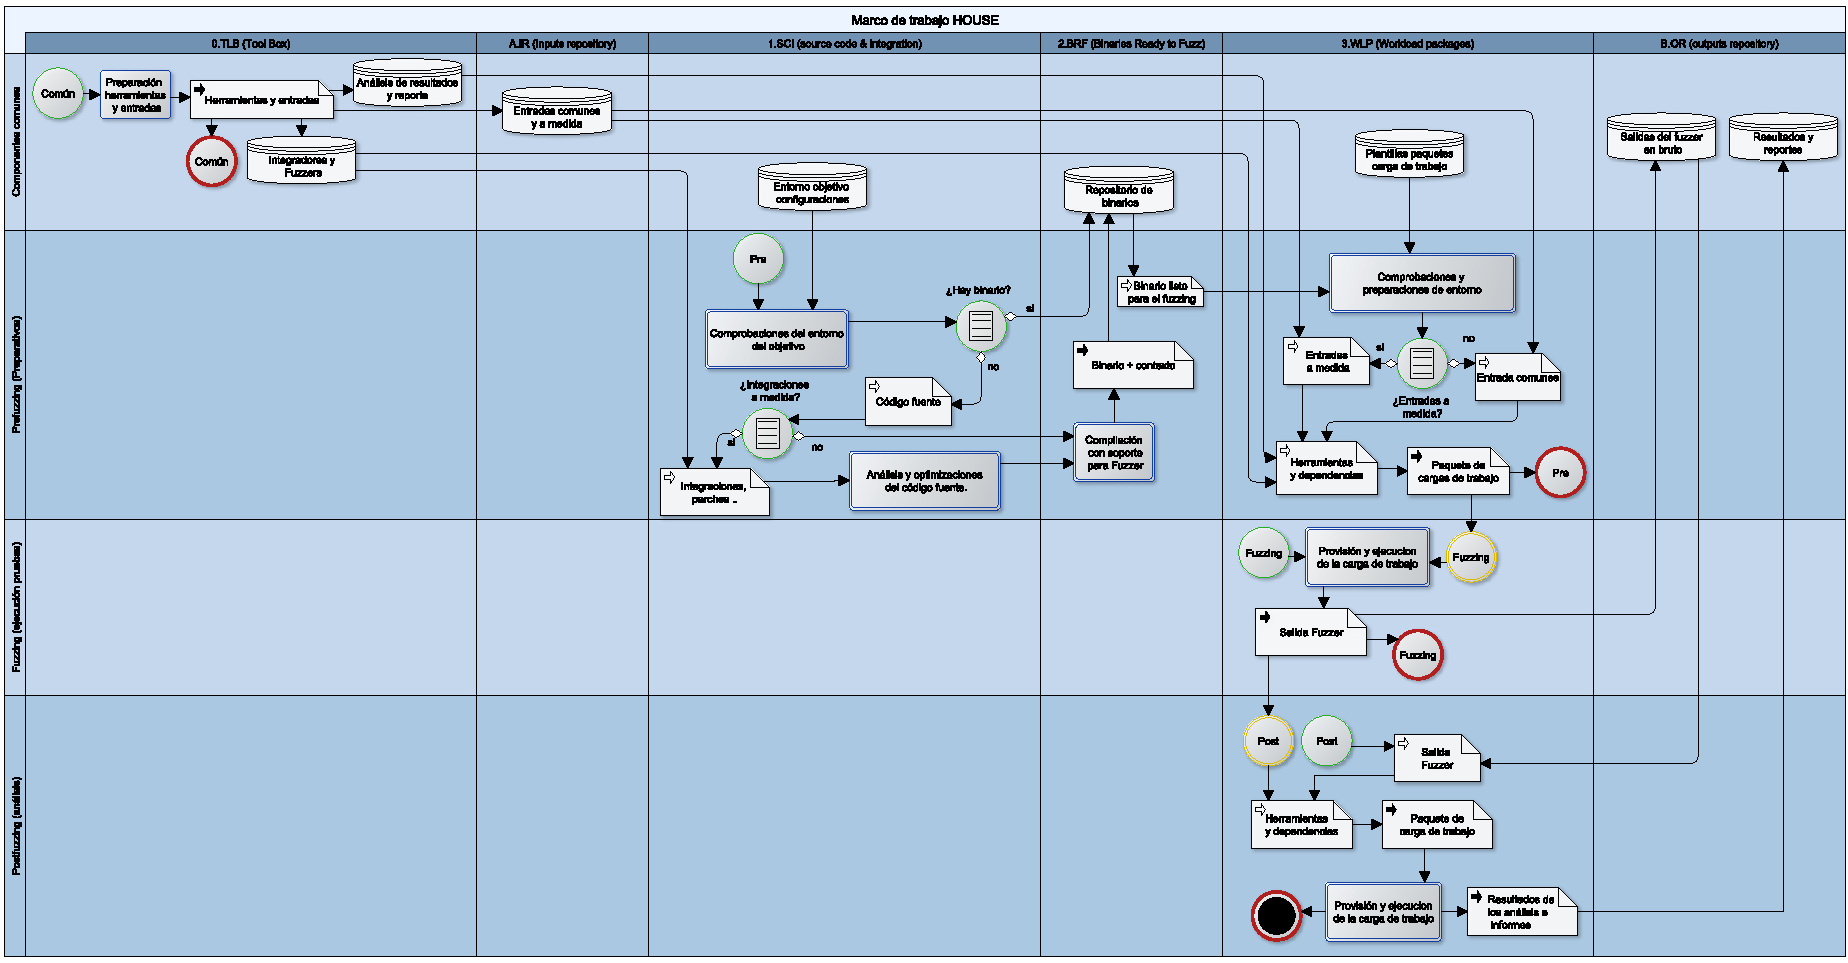
\includegraphics[scale=0.41]{./figures/data/Tabla_procesos_v5_ES _horizontal.pdf} 
    \end{column}
 \end{columns}
%%%\begin{figure}[htbp]
\begin{figure*}[ht!]
    %%\centering
    %%\centerline{
    
    %%% El EPS se carga las tranparencias
    %%\includegraphics[width=0.9\textwidth]{./figures/Tabla_procesos_simplificada_paper.eps}
    %%\includesvg[width=0.9\textwidth]{./figures/Tabla_procesos_simplificada_paper.svg}}
    %%\includesvg[width=1.5\textwidth]{./figures/Tabla_procesos_simplificada_paper.svg}
    
    %%\resizebox{1.5\textwidth}{!}{\includesvg{./figures/data/Tabla_procesos_simplificada_paper.svg}} %%% version simplificada
    \resizebox{1.5\textwidth}{!}{\includesvg{./figures/data/Tabla_procesos_v5.svg}} %%% version detallada
    
    %%}
    
    \caption{Diagrama BPMN marco de trabajo HOUSE.}
    \label{fig:tabla_procesos}

%%\end{figure}
\end{figure*}
   
}
\end{frame}
% ---- DIAPOSITIVA ----
% * 4 diapositivas (una por cada una de las "fases"/procesos). Por ejemplo, haciendo zoom al BPMN global, por inicio, fin, proceso intermedio por fases/procesos.
\begin{frame}{Flujo de trabajo: Fase 1 - Común}
\only<1>{
\centering
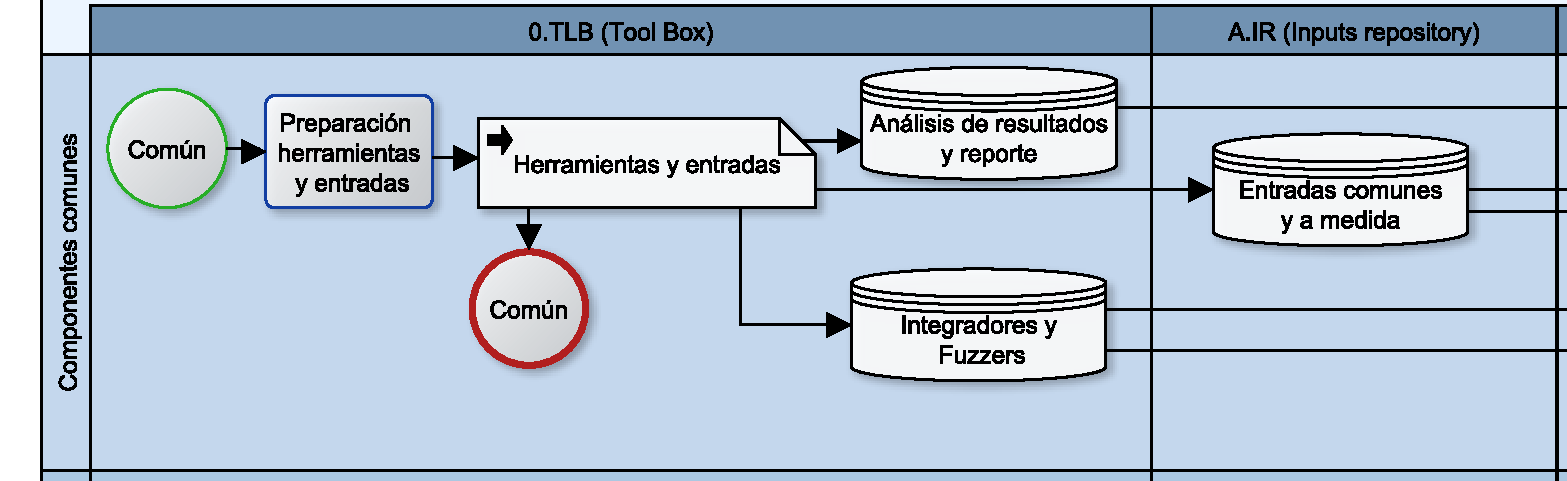
\includegraphics[scale=0.45]{./figures/data/Tabla_procesos_v5_ES _horizontal_Fase_1.pdf} 
}
\end{frame}
\begin{frame}{Flujo de trabajo: Fase 2 - \textit{Prefuzzing}}
\only<1>{
\centering
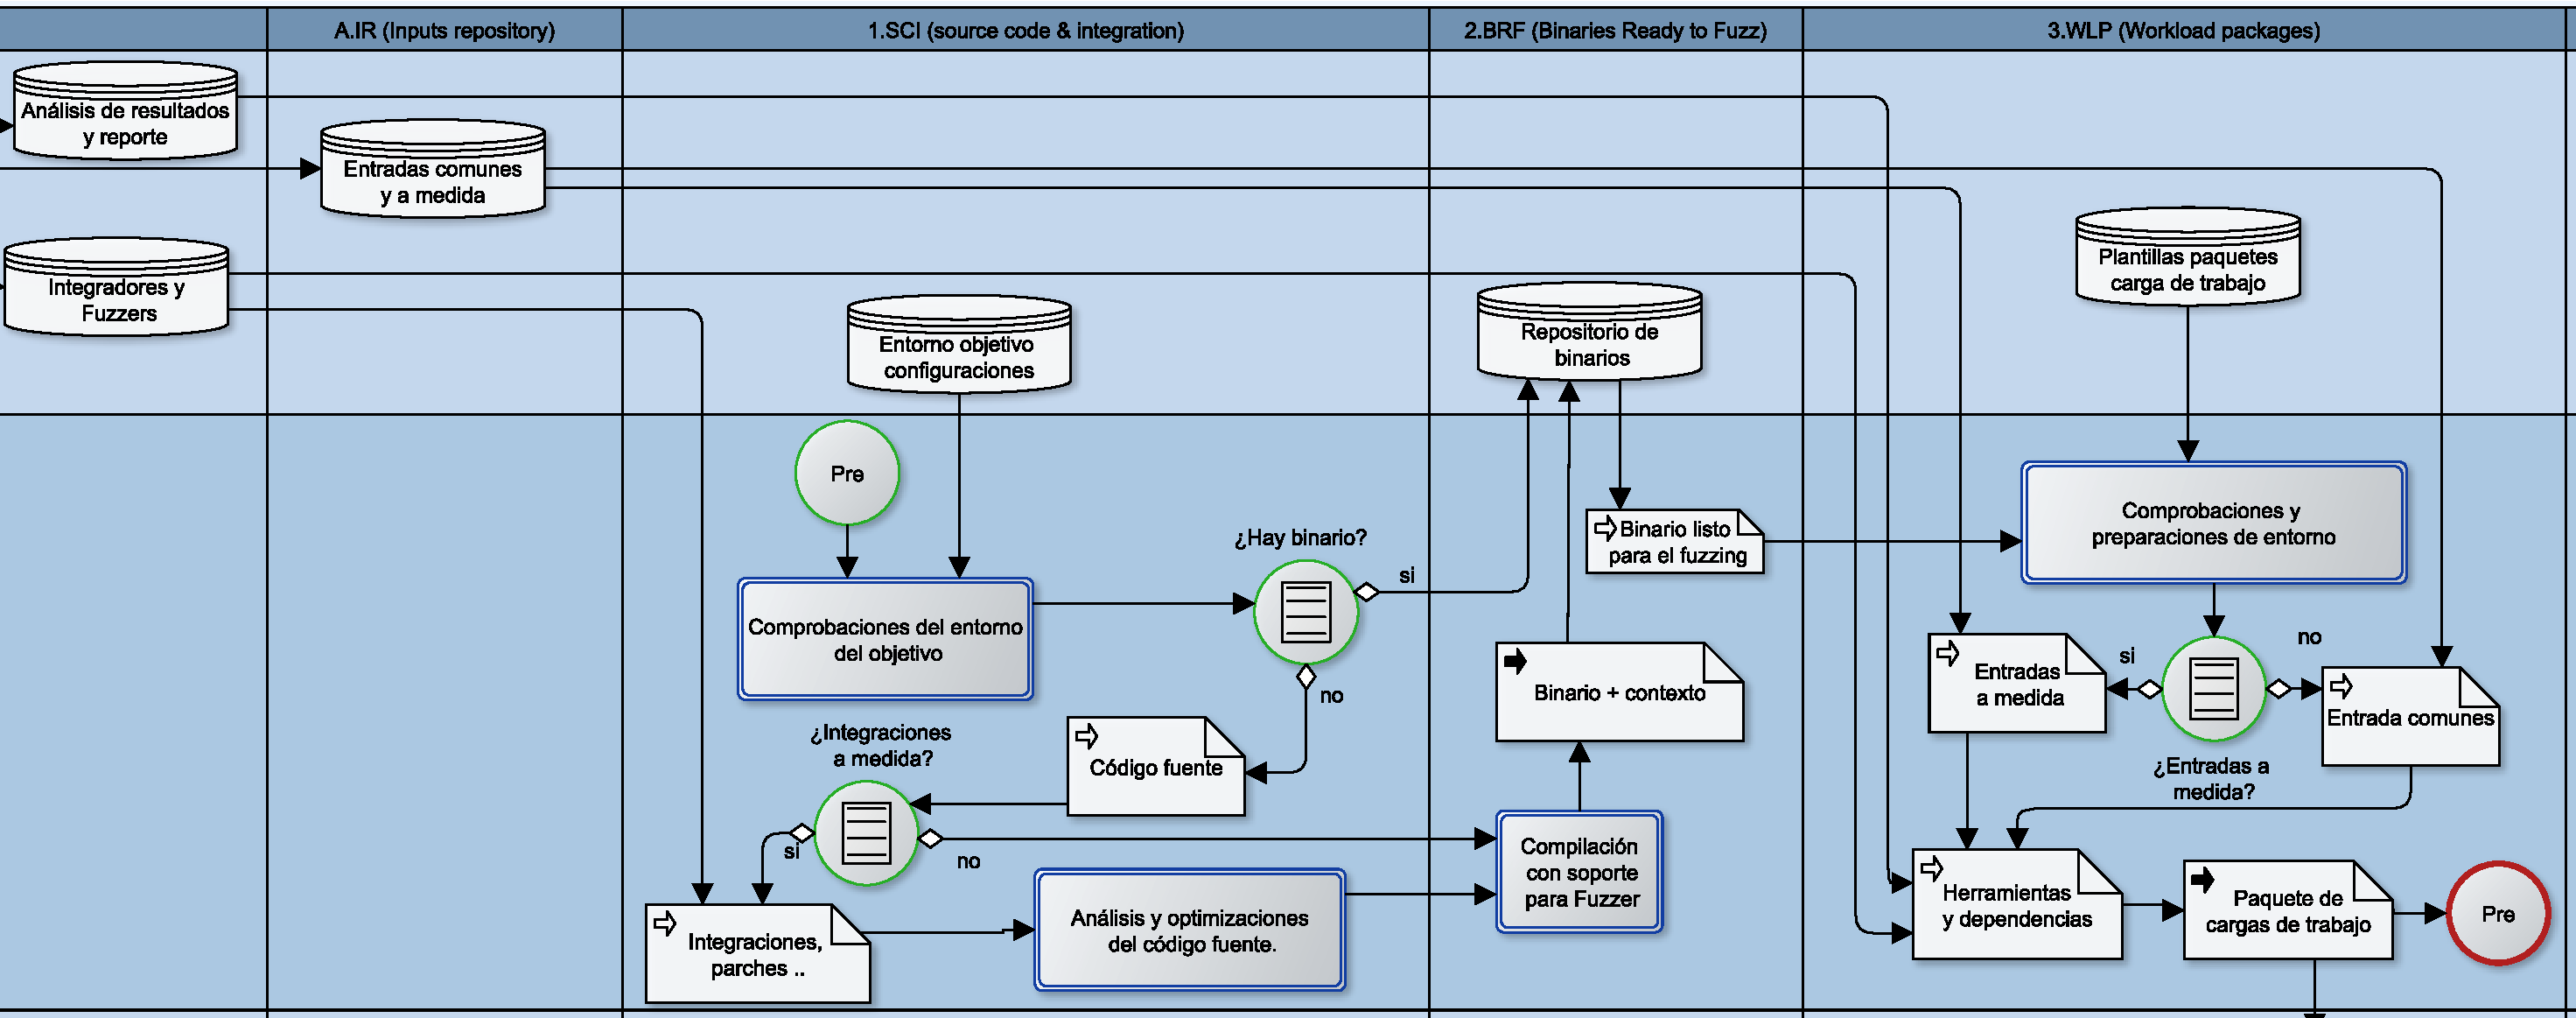
\includegraphics[scale=0.25]{./figures/data/Tabla_procesos_v5_ES _horizontal_Fase_2.pdf}
}
\end{frame}
\begin{frame}{Flujo de trabajo: Fase 3 - \textit{Fuzzing}}
\only<1>{
\centering
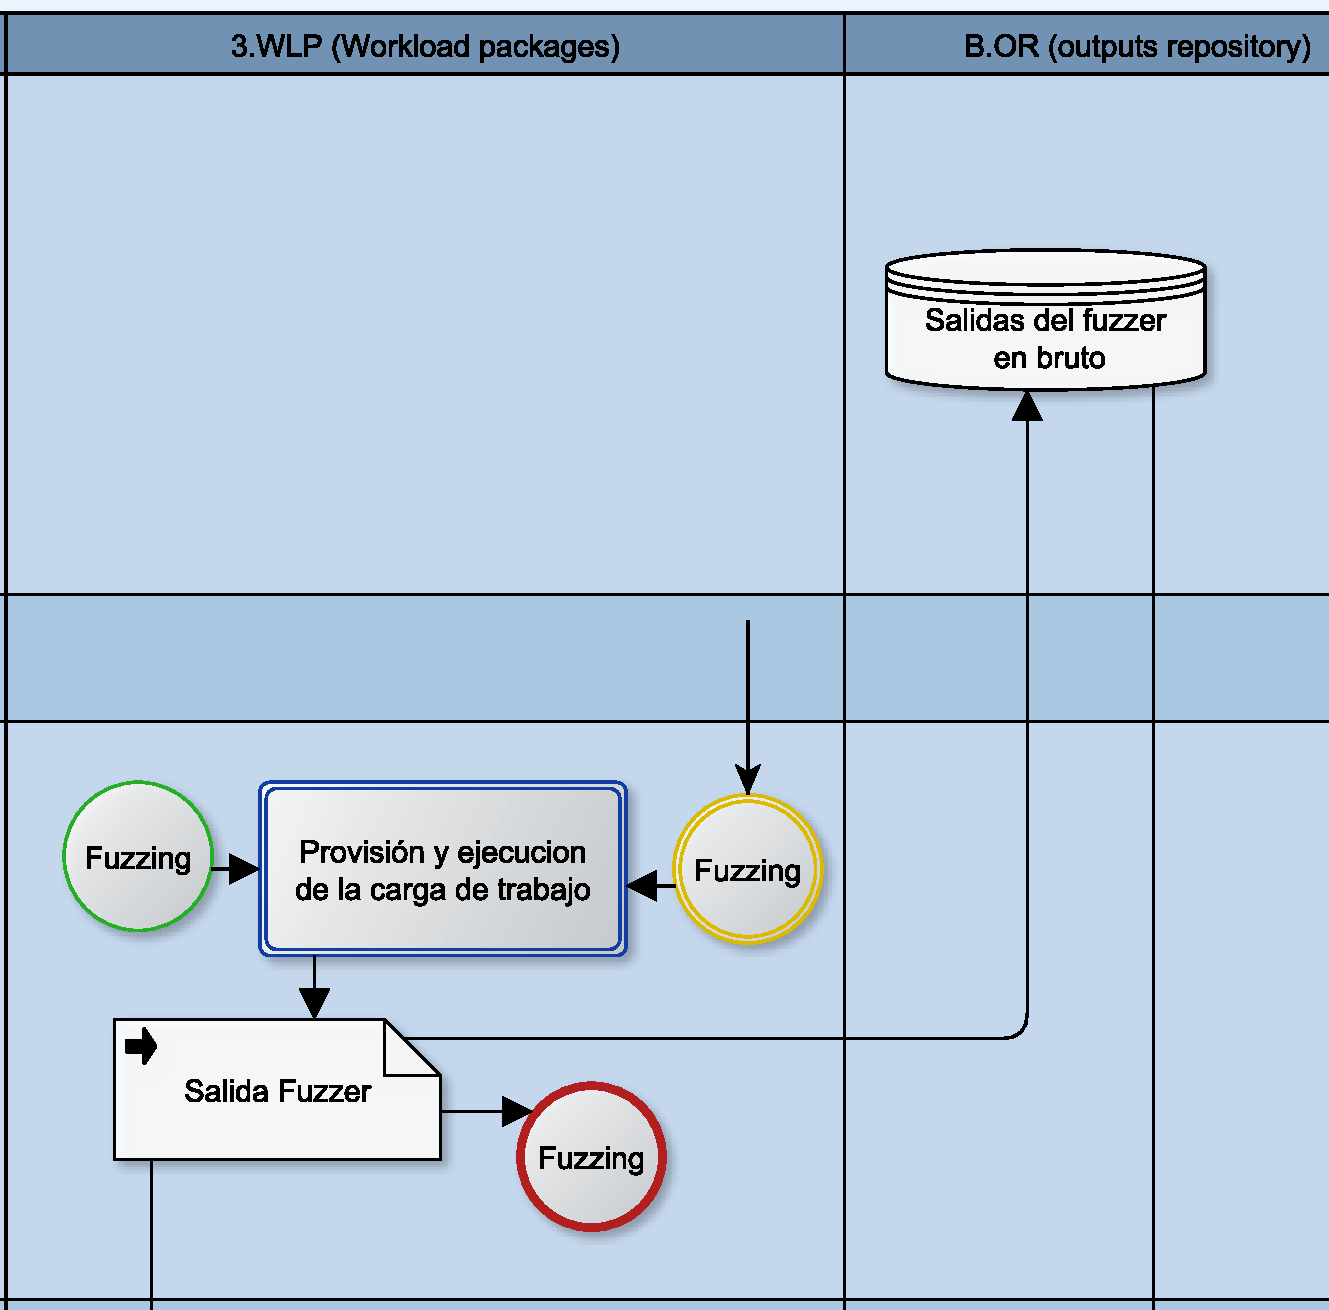
\includegraphics[scale=0.30]{./figures/data/Tabla_procesos_v5_ES _horizontal_Fase_3.pdf}
}
\end{frame}

\begin{frame}{Flujo de trabajo: Fase 4 - \textit{Postfuzzing}}
\only<1>{
\centering
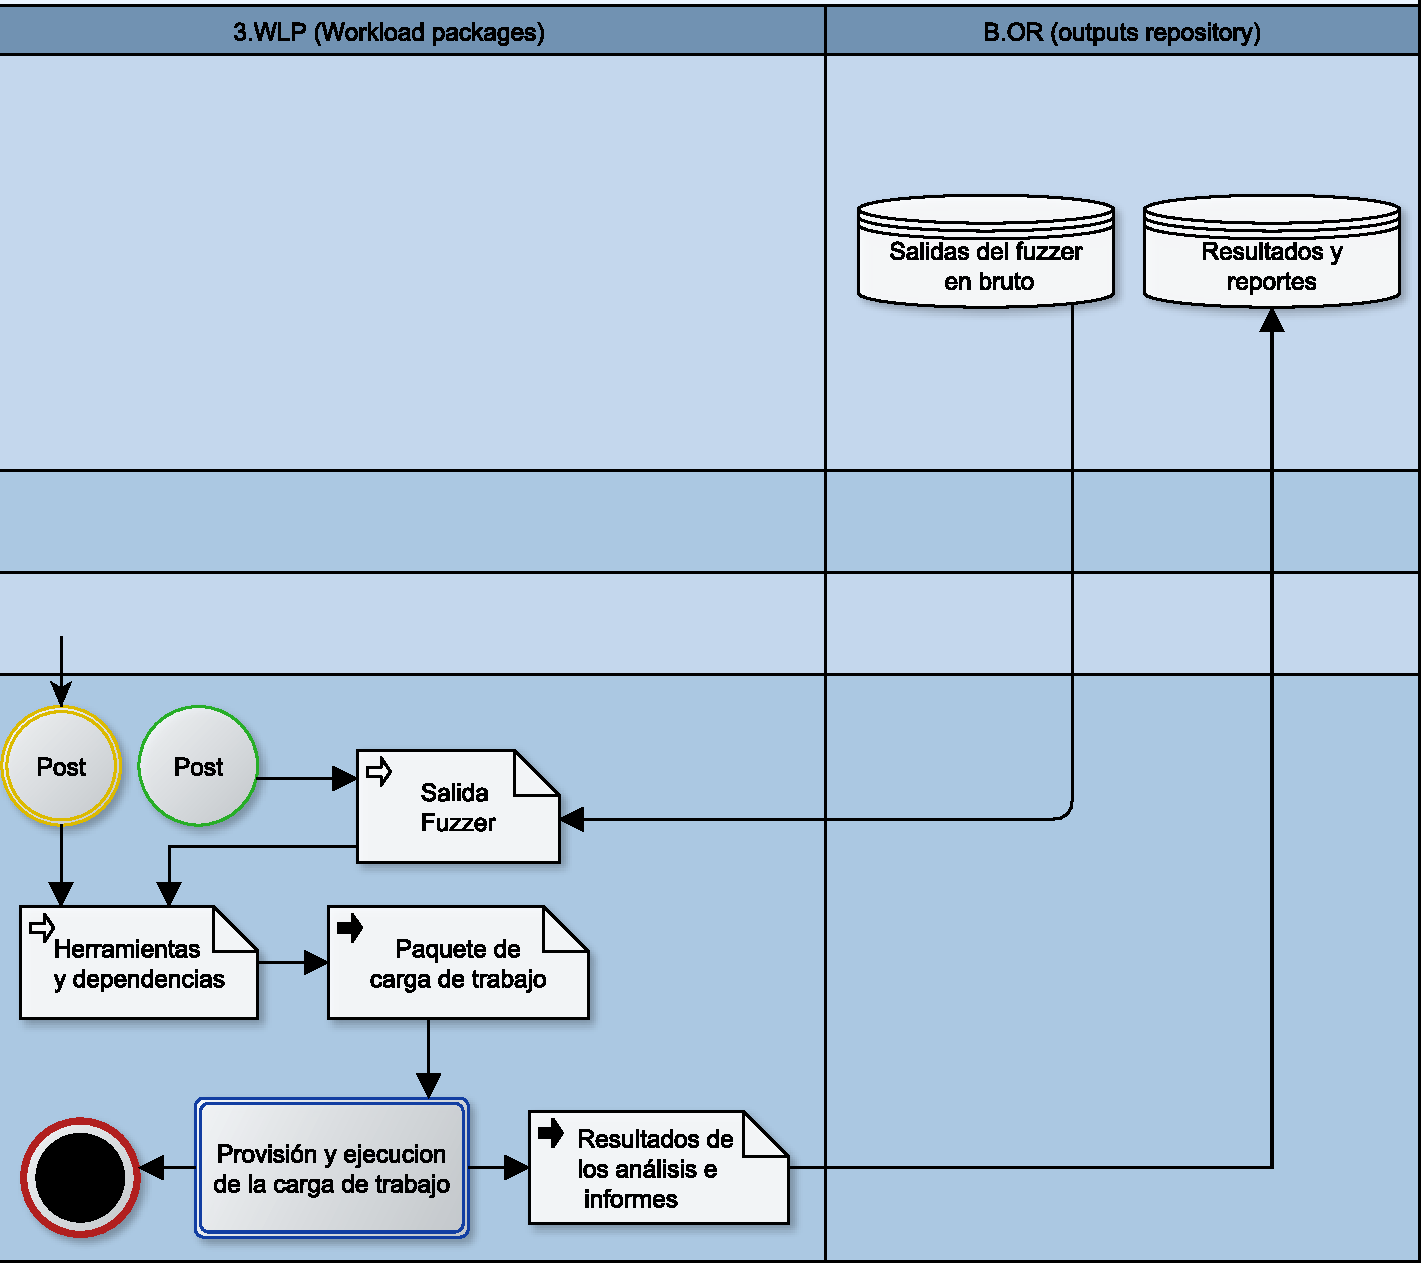
\includegraphics[scale=0.30]{./figures/data/Tabla_procesos_v5_ES _horizontal_Fase_4.pdf}
}
\end{frame}

% ***************************************************************************
\section{Resultados y discusión}
\frame{\sectionpage}

\begin{frame}{Prueba de concepto - Entorno}
%% ¡¡¡¡ Importante es lo que da valor al trabajo presentado !!!!

\only<1>{
% ---- DIAPOSITIVA ----
% * Descripción de la prueba (scripts Slurm, AFL++, white-box, binarios, etc)
% Referencia al repositorio github.
% ---------------------
    \begin{columns}

        \begin{column}{0.45\textwidth}
      \begin{itemize}
            \item HPC Caléndula.
               \begin{itemize}
            \item Arquitecturas Intel, Cascade Lake y Haswell.
            \item Sistema operativo CentOS 7.7
            \item Políticas de seguridad y requisitos del \textbf{ENS}.
            \item Slurm como sistema de gestión de cargas de trabajo.
                \end{itemize}
            \end{itemize}
             \begin{itemize}
             \item Limitaciones y características.
             \begin{itemize}
            \item 50 trabajos máximo.
            \item Nodos estándar del HPC.
            \item Nodo debug.
    \end{itemize}
    \end{itemize}
            \end{column}
            \begin{column}{0.45\textwidth}
            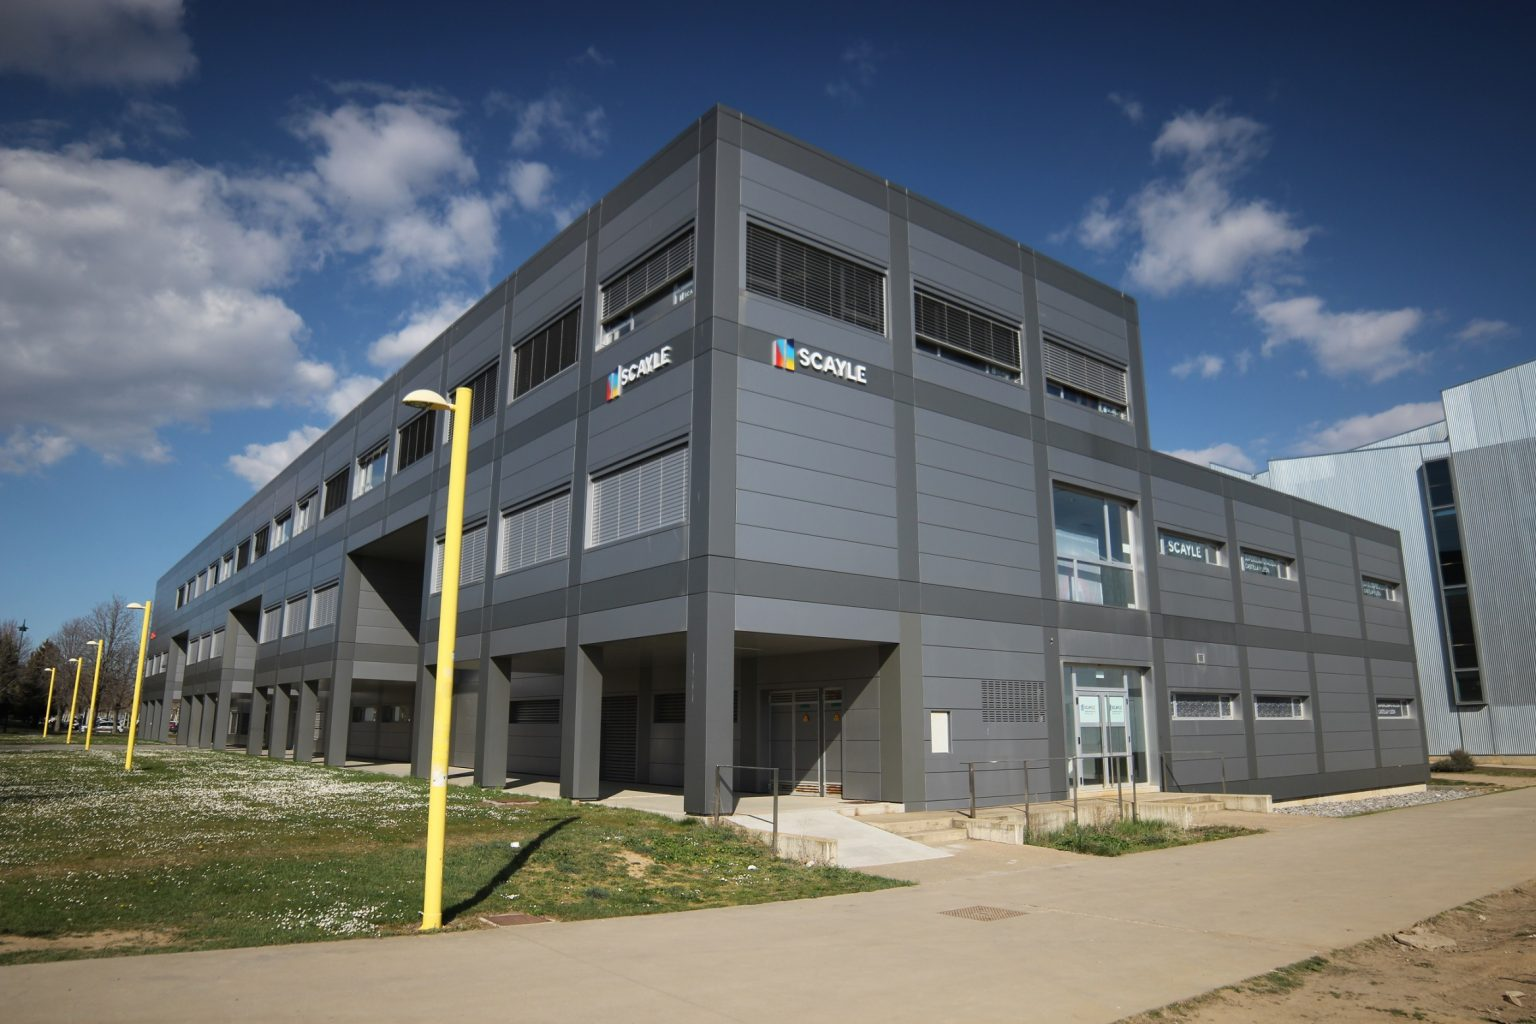
\includegraphics[width=\linewidth]{./img/Scayle-foto-exterior.jpg}
            \end{column}

  \end{columns}
}
\end{frame}
\begin{frame}{Prueba de concepto - Características y logros}
\only<1>{

      \begin{itemize}
            \item Desarrollo de scripts para Slurm para gestionar con cargas de trabajo las distintas fases.
            \item Implementar casos de uso básicos con el \textit{fuzzer} AFL$++$.
            \item Instrumentación con afl-gcc.
            \item Tipo {\fz}: \textit{white-box} de cobertura de código.
            \item PUT: \texttt{date} y \texttt{expr} de la colección de utilidades coreutils.
            \item Caso básico de control: Buffer Overflow.
            \item Entrada de datos para automatizaciones: Entrada estándar (stdin)
            \item Minimizar o prescindir de adaptación de los nodos o crear nuevos perfiles software.
\end{itemize}
}
\end{frame}

\begin{frame}{Prueba de concepto - Dificultades}
\only<1>{
% ---- DIAPOSITIVA ----
% * Descripción del entorno HPC en el que se ejecuta
% * Problemas asociados: Paquetes y dependencias, singularity, contenedores, orquestación con ¿junyper?, chroot, paths/enviroments uso de modules ...
% ---------------------
\begin{itemize}
\item Las principales dificultades identificadas son:

\begin{itemize}
            \item Limitaciones de uso de herramientas basadas en ASAN en 64bits.
            \item Monitorización de \textit{crashes} usando ABRT.
            \item Librerías dinámicas del sistema.
            \item Rutas estáticas definidas en compilación.
            \item Protecciones de seguridad sistema operativo.
\end{itemize}
\end{itemize}
}
\end{frame}
\begin{frame}{Prueba de concepto - Experimentos}
\only<1>{
\begin{itemize}
\item El desarrollo de la investigación se han probado otros enfoques:
\begin{itemize}
            \item Uso de ASAN para binarios de 32bits.
            \item Junyper notebook como gestor de cargas de trabajo medio de playbooks en python.
            \item Uso de contenedores singularity.
            \item Uso chroot en espacio de usuario con PRoot - Termux
            \item Uso de \textit{modules} para gestión del entorno del sistema operativo.
\end{itemize}
\end{itemize}

}
\end{frame}
\begin{frame}{Prueba de concepto - Estado y antecedentes}
\only<1>{
% ---- DIAPOSITIVA ----
% * Problemas encontrados a la hora de ejecutarlo en Caléndula.
% Fotos ejecución.
% ---------------------
    \begin{columns}

        \begin{column}{0.45\textwidth}
        \begin{itemize}
    \item Inicialmente se trató de replicar el experimento \cite{HPC_fuzzing} usando instrumentación con GCC adaptado a un entorno HPC moderno, y una versión derivada de AFL reciente.
 
 \item Actualmente se está trabajando en la adecuación de instrumentación LLVM y se planea añadir el soportar otras arquitecturas con QEMU.
 \end{itemize}
      \end{column}

      \begin{column}{0.50\textwidth}
      \begin{figure}[htbp]
     \centering
    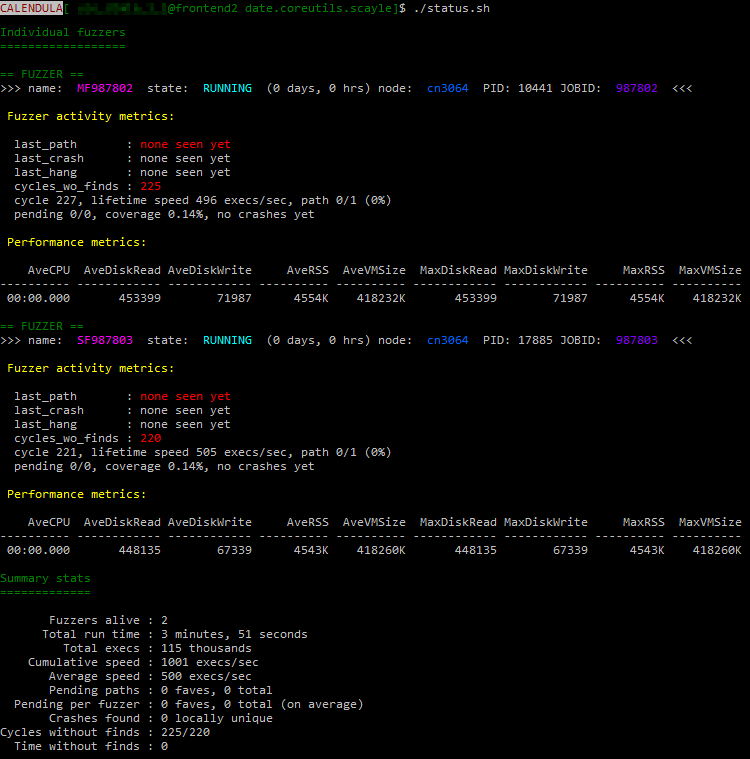
\includegraphics[width=1.0\textwidth]{./figures/data/Image_fuzzer_status_HOUSE.png}
    %\caption{Ilustración status de los trabajos de fuzzing.}
    \label{img:fuzzer_status}
\end{figure}

            \end{column}

  \end{columns}
}
\end{frame}

% ***************************************************************************
\section{Conclusiones}
\frame{\sectionpage}

\begin{frame}{Conclusiones}

% ---- DIAPOSITIVA ----
% * Resumir brevemente en 4 ó 5 puntos la sección.
% Lo del paper en itemizes.
% ---------------------
   \begin{itemize}
\item El {\fz} está cobrando cada vez más protagonismo como actividad para garantizar la calidad y la seguridad del software.
\item Grandes empresas y organizaciones se suman al {\fz} para poner en valor sus desarrollos o servicios de forma comercial.
\item Los desarrollos con intereses privados  y servicios comerciales  alrededor del {\fz} provocan dependencia tecnológica y suponen un riesgo a la confidencialidad de la información para su adopción en un ciclo de desarrollo seguro.
\item HOUSE propone un modelado del flujo de trabajo del {\fz} caracterizado por tener un enfoque abierto y agnóstico a las herramientas.
\item HOUSE permite resolver o simplificar las tareas más tediosas y complejas relacionadas con la aplicación de técnicas de {\fz}.
\end{itemize}

\end{frame}

% Cierre
% ***************************************************************************
\appendix

\begin{frame}[plain,noframenumbering]{}

\vspace{3cm}
\qquad\Huge{\color{LUCopper}{\textbf{Gracias por su atención}}}
\vspace{1cm}
\hspace{2cm}
\small{\begin{figure}[b]

\includegraphics[width=1cm]{PresentacionJNIC/figures/data/GitHub-Mark-120px-plus.png}~
\href{https://github.com/b0rh/HOUSE}{\color{blue}{https://github.com/b0rh/HOUSE}}
\end{figure}}

\end{frame}

% REFERENCIAS
% ***************************************************************************
\begin{frame}[allowframebreaks]{Referencias }
% TODO: Quitar I al final de referencias

    \bibliographystyle{apalike}
    %\bibliographystyle{IEEEtran}
    \bibliography{bibliography.bib}
\end{frame}



\end{document}
